\documentclass[11pt, fullpage,letterpaper]{article}

\usepackage[margin=1in]{geometry}
\usepackage{url}
\usepackage{amsmath}
\usepackage{float}
\usepackage{graphicx}
\usepackage{times,amsmath,amsthm,amsfonts,eucal,graphicx}
\usepackage{hyperref}

\newcommand{\assignmentId}{1}

\newcommand{\bx}{{\bf x}}
\newcommand{\bw}{{\bf w}}

\renewcommand{\cite}[1]{[#1]}
\def\beginrefs{\begin{list}%
        {[\arabic{equation}]}{\usecounter{equation}
         \setlength{\leftmargin}{2.0truecm}\setlength{\labelsep}{0.4truecm}%
         \setlength{\labelwidth}{1.6truecm}}}
\def\endrefs{\end{list}}
\def\bibentry#1{\item[\hbox{[#1]}]}



\title{Biodiversity Clustering}
\author{Jadon Wagstaff and Christian Felt}

\begin{document}

	\maketitle
	
	\section{Introduction}
		Data was obtained from the International Union for the Conservation of Nature (IUCN) via shapefiles [IUCN 17]. The files contained sets of polygons representing the ranges of different species assessed by the IUCN. We set out to explore methods of polygon clustering, and how we could use clustering to answer the questions:
		\begin{itemize}
			\item Where are areas of high biodiversity?
			\item Where are areas of high levels of species endangerment?
		\end{itemize} 
		We divided the work into two parts. Christian created centroids of each polygon and implemented clustering algorithms discussed in class. Jadon created a point cloud for the data, and explored density based clustering methods.
	
	\section{Data}
		The data obtained was in the form of Esri shapefiles containing polygons. Each polygon was associated with a species identification number. These polygons were often large, diverse, complex, and overlapping. They proved to be unsuitable for our methods as they were. The first method used to mitigate these problems was to calculate centroids of the polygons using ArcMap software. The other method was to create an ordered set of points on the globe and find which were contained in the polygon, then use this point cloud for the clustering algorithms.
		
		To create a point cloud, we created an array of size $n$ with each row corresponded to a latitude from $-89.8^o$ to $89.8^o$ with a change of $.2^o$ latitude between each row. Each array contained an array of longitude elements from		 $-180^o$ to $180^0$ in increments of $\frac{.2}{\cos(latitude)}$. This gave about a million points in a grid like point cloud set with approximately $22km$ great-circle distance between adjacent points. For a given polygon, each point was assessed to determine whether it was contained in the polygon or not. This was accomplished by determining how many times a ray, starting at the point, intersected the polygon. Once it was determined that a point was in the polygon, the species id of that polygon was added to an array representing that point. This was done for all polygons and the result was an ordered point cloud, each an array of species found at that geographical coordinate. Each array has the property that the size of the array corresponds to the depth of polygons at that point. This set of points preserves more information about the shape and size of the polygon than centroids, and the fact that the point cloud is ordered was utilized to make the clustering algorithms more efficient.
		
		Another shortcoming of the data is that information about red-list status was missing. (Red-list status is essentially whether a species is endangered or not.) To supply the needed information, the IUCN database was queried for each species represented by polygons. After that the clustering algorithms were able to do clustering on the whole data set, or just polygons associated with species on the red-list. 
	
	\section{Class Methods}
		Using ArcMap software, I computed the centroids of the polygons that represent the ranges of terrestrial mammal, reptile, and amphibian species in the IUCN shapefiles. Using my own Python code, I turned the latitude and longitude coordinates of these centroids into a 2-dimensional matrix and performed various kinds of clustering, trying to find areas of especially high density of endangered species.
	
		To measure distance, I used the great-circle distance as given by d from the Haversine formula, where $\phi$ latitude, $\lambda$ is longitude, and $R$ is the radius of the earth.
		\begin{equation}
			a = \sin^2 \frac{\Delta\phi}{2} + \cos \phi_1 (\cos \phi_2)  (\sin^2 \frac{\Delta\lambda}{2})
		\end{equation}
		\begin{equation}
			c =  \begin{cases} 
					0 & a = 0 \cr \tan^{-1}{\frac{\sqrt{1-a}}{a}} & a \neq 0
				\end{cases}
		\end{equation}
		\begin{equation}
			d = R*c
		\end{equation}
	
		Since the Earth is not perfectly spherical, the great-circle distance may be wrong by up to approximately 0.3\% or 22km according to the analysis at http://gis.stackexchange.com/q/25494. In their article “Global Patterns of Terrestrial Vertebrate Diversity and Conservation,” Jenkins et al set 100km as a reasonable lower limit for “fine-grained spatial analysis” in this field.
	
		Hierarchical clustering ran too slowly for the full dataset (74,529 points) or for amphibians alone (18,694 points). K-means++ worked for small numbers of clusters (20 or less) but became obnoxiously slow for larger k. Lloyd’s was also too slow for more than about 20 clusters.
	
		Gonzalez clustering processed the entire dataset in less than 10 seconds. Using the “elbow” principle, I chose k=40 (see Figure 1). The resulting clusters (see Figure 2) seem surprisingly reasonable, often lining up with the “25 Global Biodiversity Hotspots” shown in Figure 3. For instance, Gonzalez gives Madagascar, New Zealand, and the Caucasus Mountains their own clusters, separates the Pacific Northwest from the rest of the Rockies, and divides up the Amazonian, Congo, and Indonesian rainforests in roughly canonical ways. Also, the Aleutian and Canary Islands, Newfoundland, and Hawaii are given their own clusters, and the Andes, Himalayas, and other mountain chains are not too broken up. 
	
		On the other hand, areas with low density of endangered species, such as Siberia or the Sahara Desert, seem to get partitioned in fairly meaningless ways. Also, my clusters assign the Mediterranean Basin, somewhat oddly, to 3 different centers. 
	
		But if my clustering inspires confidence by reflecting the common knowledge in some areas, then perhaps where it deviates from the usual boundaries, the results should not be immediately dismissed. They might provide questions for further research. For instance, is there really a significant difference in the species and habitats of the western half of the Mediterranean Basin versus the half that lies to the east of Sicily? What (if anything) justifies the separation of India from Indochina, Scotland from the rest of the U.K., or the area along the coast of West Africa from the Congo River Basin at a right angle to the south?
	
	\section{Density Based Clustering}
		In this section, we ask ''Where are areas of high biodiversity?'' and ''Where are areas of high levels of species endangerment?'' Since we are asking to find where areas of greater biodiversity are located, a density based clustering algorithm is a natural choice. Additionally, a paper on the topic \cite{Joshi 11} gives evidence that density based algorithms are good option for solving polygon clustering problems. Using the centroid data, the Haversine distance metric, and suggestions from the paper \cite{Joshi 11}, an implementation of a modified version of dbscan was created in C++.
		\begin{tabbing}
			Mod\= ifie\= d db\= scan algorithm:\\
			\> Choose distance $\epsilon$ and number of points $minPts$\\
			\> Go to each data point and if it is unlabelled\\
			\> \> If the number of data points within $\epsilon$ is less than $minPts$\\
			\> \> \> label it outlier\\
			\> \> otherwise\\
			\> \> \> label it and all reachable core points as part of the same cluster\\
		\end{tabbing}

		A core point is a point with greater than $minPts$ number of points within an $\epsilon$ radius. This implementation differs from the normal dbscan because points are only included in a cluster if they qualify as a core point and they are within $\epsilon$ of a core point in the cluster. Run-time for the implementation on all  74,529 centroids was about half an hour. This implementation created clusters; however, the high density clusters do not match well with the diversity maps found on biodiversitymapping.org. This is the result of the centroid data losing too much information about the polygons.
		
		To improve results, an implementation of the modified dbscan for the ordered point cloud dataset was created. For this implementation, the density of an $\epsilon$ radius around a point $p$ was found by taking the average depth of $p$ and each point within $\epsilon$ of $p$. Also, $\epsilon$ was limited to values greater than $22km$ since no points were closer together than that. The resulting clusters matched nicely with maps on biodiversitymapping.org as long as $\epsilon$ was smaller than about $100km$.
		
		At this point, the polygons were able to be clustered for some depth threshold to provide regions where biodiversity or endangerment were above that threshold. Additionally, the depth information can be used to create a heat map of biodiversity or endangerment. These are interesting, if somewhat trivial, tools to analyse the data. Now, is there a way to find and quantify the regions of high density relative to their surroundings? The next section addresses this question.
		
	\section{Density Based Cluster Persistence}
		In topological data analysis, persistent homology is used to detect prominent features of a space and the results are shown in a persistence diagram. The ideas found in persistent homology can be adapted to find regions of high density relative to their surroundings. Instead of building complexes by increasing the $\epsilon$ ball around a point, clusters are built by decreasing the $minPts$ value and keeping $\epsilon$ constant. And instead of killing complexes by merging them into older complexes, clusters are killed by merging them with deeper clusters.
		
		\begin{tabbing}
			Mod\= ifie\= d db\= scan \= alg\= orithm with persistence calculation:\\
			\> choose distance $\epsilon$ and the maximum possible points, $max$, within any $\epsilon$\\
			\> for $minPts = max..0$\\
			\> \> for each point $p$, if $p$ is unlabelled and a core point\\
			\> \> \> let $p$ and all reachable core points be in set $C$\\
			\> \> \> \> if all points in $C$ are unlabelled\\
			\> \> \> \> \> for cluster $c$, $birth(c) \leftarrow minPts$\\
			\> \> \> \> \> $\forall p_i \in C$, $label(p_i) = c$\\
			\> \> \> otherwise, choose $p_0 \in C$ s.t. $birth(p_0)$ is maximal\\
			\> \> \> \> for any labelled $p_i \in C$, if $label(p_i) \neq label(p_0)$\\
			\> \> \> \> \> $death(label(p_i)) \leftarrow minPts$\\
			\> \> \> \> \> $\forall p_i \in C$, $label(p_i) \leftarrow label(p_0)$\\
		\end{tabbing}
		
		All the clusters $c$ produced by the algorithm have a point, $(birth(c), death(c))$, that can be plotted on a $max(minPts) \times max(minPts)$ size graph.  to form a persistence diagram. Clusters with a high birth value are more dense than clusters with lower birth values. Further, $death(c)$ gives the lowest density that occurs between that point and the closest denser cluster. These can be used to find the prominence of a density cluster which is the distance between $(birth(c), death(c))$ and the diagonal. The results for mammal biodiversity are shown in the figures below. For each cluster, a point was generated by calculating the mean latitude and longitude for all points in the cluster at birth. The points corresponding to interesting points on the persistence diagram are shown on the map.
		
		\begin{figure}[H]
			\centering
			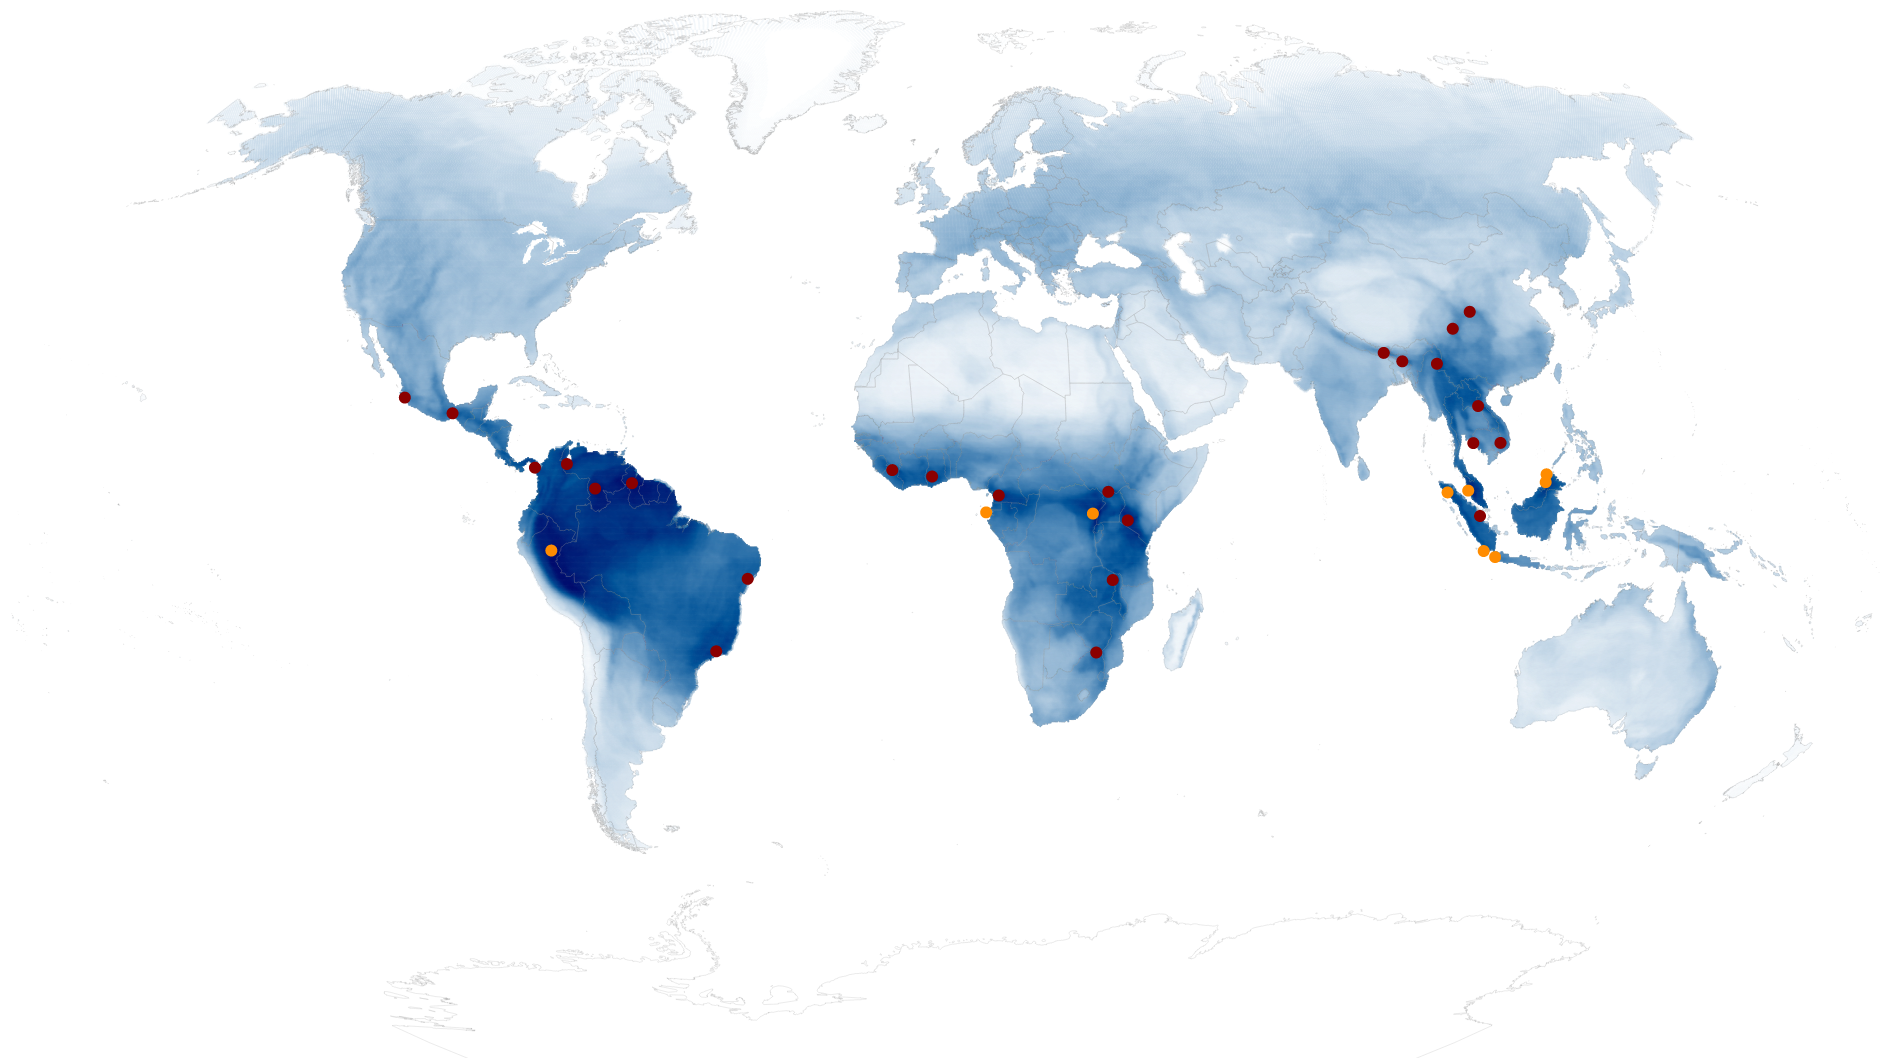
\includegraphics[width=20cm]{map.png}
			\caption{Heat map showing mammal density. Generated from depth of points on a grid overlaying the earth.}
		\end{figure}
		
		\begin{figure}[H]
			\centering
			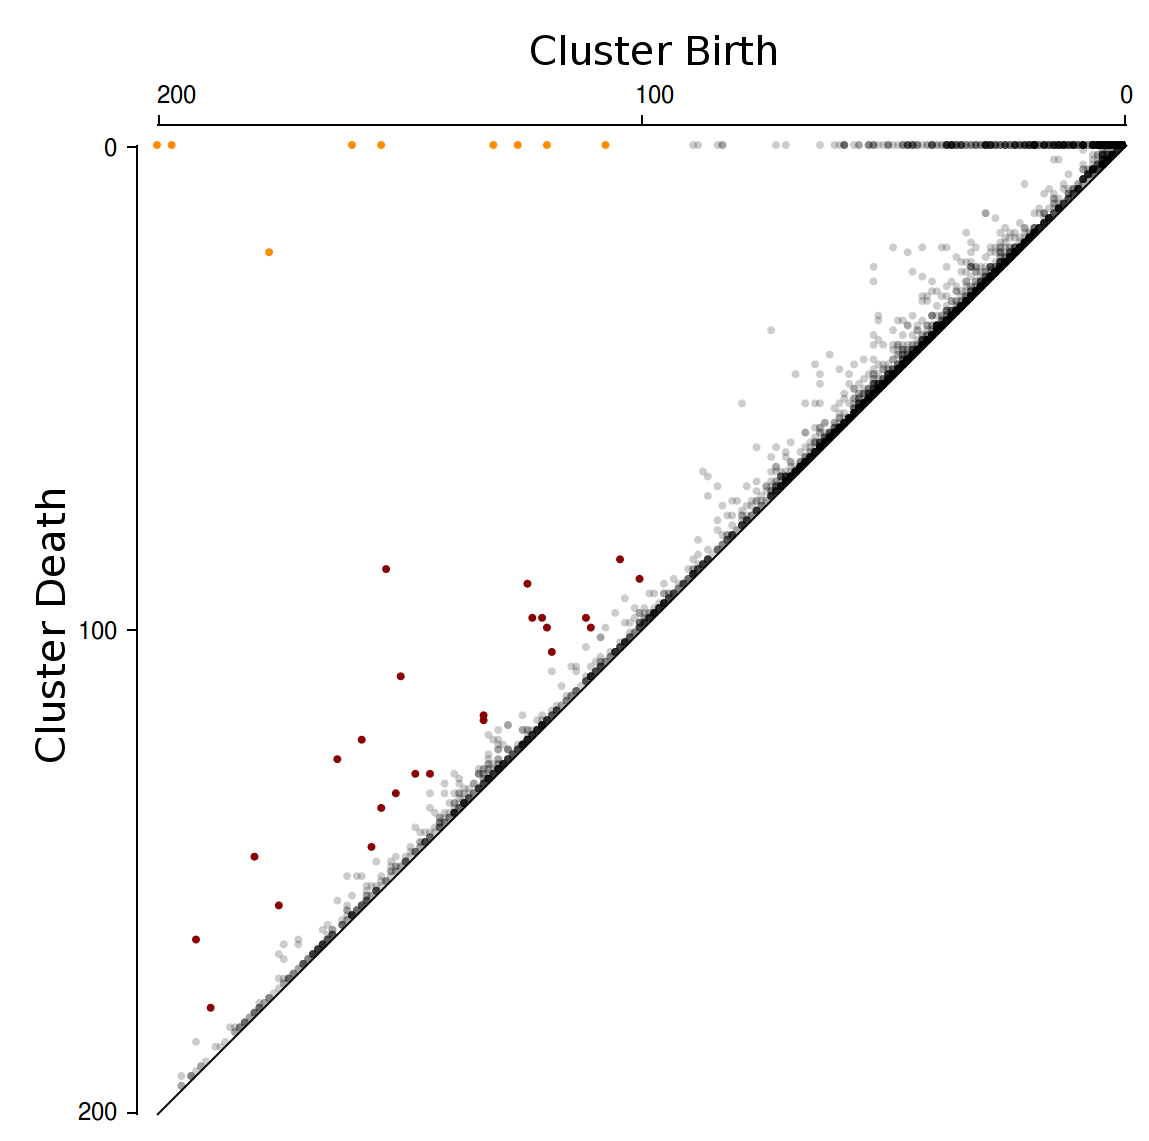
\includegraphics[width=10cm]{graph.png}
			\caption{Persistence diagram of mammal density. Orange points have both high density $>100$ and high prominence $>75$. Red points have high density $>100$ and less prominence $<75$, $>10$.}
		\end{figure}
		
	

		\pagebreak
	
	\section*{References}
		\beginrefs

			\bibentry{IUCN 17} International Union for the Conservation of Nature. (2017) \emph{Spatial Data Download}. Retrieved from http://www.iucnredlist.org/technical-documents/spatial-data/

			\bibentry{Joshi 11} Joshi, D. (2011). Polygonal spatial clustering.  \emph{Computer Science and Engineering: Theses, Dissertations, and Student Research}, 16.

		\endrefs
	

		
		
	
	
\end{document}